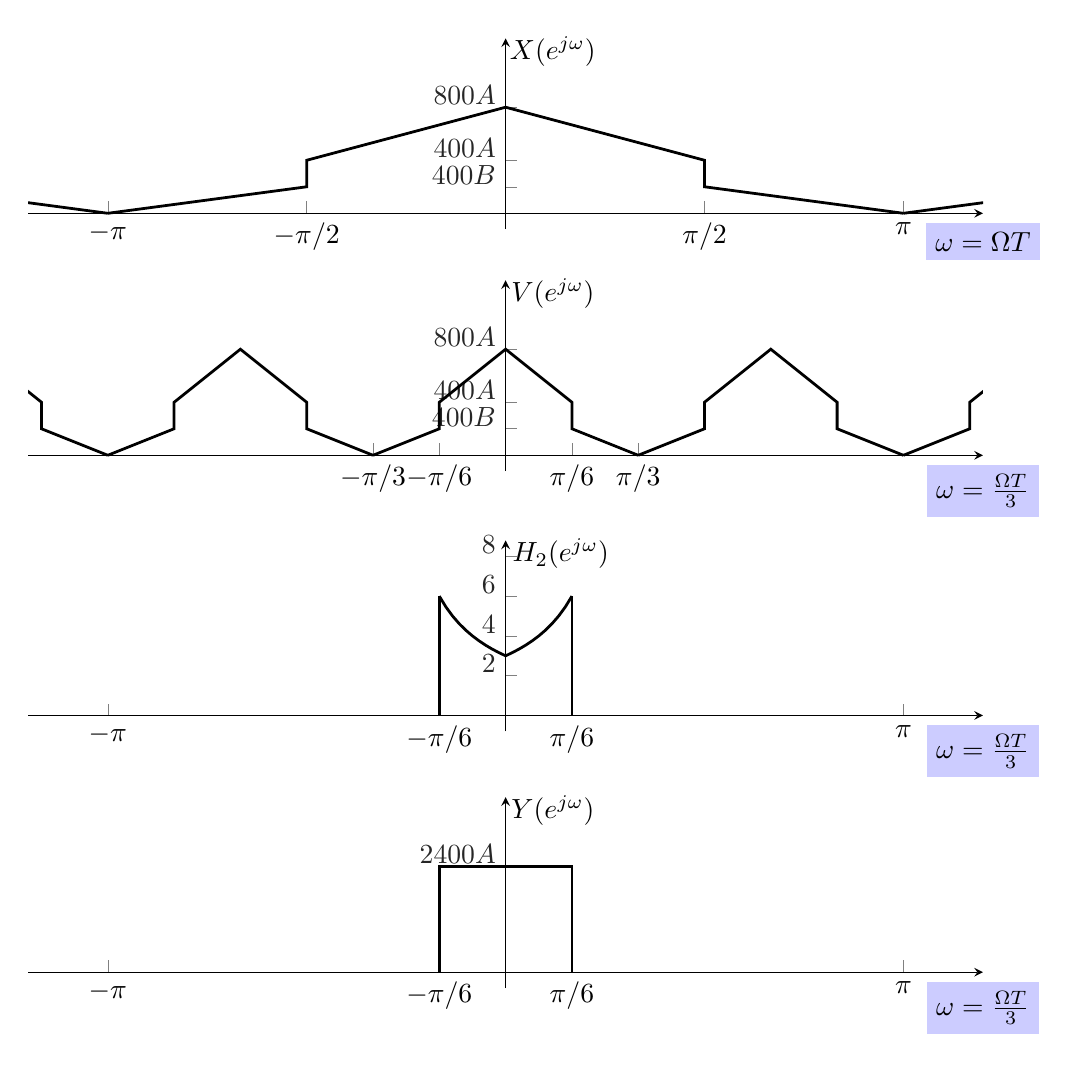
\begin{tikzpicture}
\begin{axis}[
name=plot1,
%at=(plot2.below south east), anchor=above north east,
axis lines*=middle,
enlargelimits = true,
clip=true,
scale only axis,
width=\textwidth,
height=0.2\textwidth,
ymin=0, ymax=3,
xmin=-8, xmax=8,
axis line style={->,>=stealth},
xlabel={\tikz[baseline]{\node[fill=blue!20,anchor=base] (t1) {$\omega = \Omega T$};}},
ylabel={$X(e^{j\omega})$},
every axis x label/.style={
	at={(ticklabel* cs:1)},
	%xshift=0.2cm,
	anchor=north,
},
every axis y label/.style={
	at={(ticklabel* cs:0.8)},
	anchor=south,
	xshift=0.6cm,
},
ytick={0.5, 1, 2},
yticklabels={$400B$, $400A$, $800A$},
yticklabel style={yshift=0.15cm},
xtick={-8, -4, 4, 8},
xticklabels={$-\pi$, $-\pi/2$, $\pi/2$, $\pi$}, 
every outer y axis line/.append style={white!15!black},
every y tick label/.append style={font=\color{white!15!black}},
legend style={draw=white!15!black,fill=white,legend cell align=left}]
\def\fs{16}
\foreach \k in {-1, 0, 1}{
	\addplot[solid, line width=1pt] coordinates {(-8+\k*\fs, 0) (-4+\k*\fs, 1/2) (-4+\k*\fs, 1) (0+\k*\fs, 2) (4+\k*\fs, 1) (4+\k*\fs, 1/2) (8+\k*\fs, 0)};	
}
\end{axis}

\begin{axis}[
name=plot2,
at=(plot1.below south east), anchor=above north east,
axis lines*=middle,
enlargelimits = true,
clip=true,
scale only axis,
width=\textwidth,
height=0.2\textwidth,
ymin=0, ymax=3,
xmin=-24, xmax=24,
axis line style={->,>=stealth},
xlabel={\tikz[baseline]{\node[fill=blue!20,anchor=base] (t1) {$\omega = \frac{\Omega T}{3}$};}},
ylabel={$V(e^{j\omega})$},
every axis x label/.style={
	at={(ticklabel* cs:1)},
	%xshift=0.2cm,
	anchor=north,
},
every axis y label/.style={
	at={(ticklabel* cs:0.8)},
	anchor=south,
	xshift=0.6cm,
},
ytick={0.5, 1, 2},
yticklabels={$400B$, $400A$, $800A$},
yticklabel style={yshift=0.15cm},
xtick={-8, -4, 4, 8},
xticklabels={$-\pi/3$, $-\pi/6$, $\pi/6$, $\pi/3$}, 
every outer y axis line/.append style={white!15!black},
every y tick label/.append style={font=\color{white!15!black}},
legend style={draw=white!15!black,fill=white,legend cell align=left}]
\def\fs{16}
\foreach \k in {-2, -1, 0, 1, 2}{
	\addplot[solid, line width=1pt] coordinates {(-8+\k*\fs, 0) (-4+\k*\fs, 1/2) (-4+\k*\fs, 1) (0+\k*\fs, 2) (4+\k*\fs, 1) (4+\k*\fs, 1/2) (8+\k*\fs, 0)};	
}

\end{axis}

\begin{axis}[
name=plot3,
at=(plot2.below south east), anchor=above north east,
axis lines*=middle,
enlargelimits = true,
clip=true,
scale only axis,
width=\textwidth,
height=0.2\textwidth,
ymin=0, ymax=8,
xmin=-24, xmax=24,
axis line style={->,>=stealth},
xlabel={\tikz[baseline]{\node[fill=blue!20,anchor=base] (t1) {$\omega = \frac{\Omega T}{3}$};}},
ylabel={$H_2(e^{j\omega})$},
every axis x label/.style={
	at={(ticklabel* cs:1)},
	%xshift=0.2cm,
	anchor=north,
},
every axis y label/.style={
	at={(ticklabel* cs:0.8)},
	anchor=south,
	xshift=0.7cm,
},
yticklabel style={yshift=0.15cm},
xtick={-24, -4, 4, 24},
xticklabels={$-\pi$, $-\pi/6$, $\pi/6$, $\pi$}, 
every outer y axis line/.append style={white!15!black},
every y tick label/.append style={font=\color{white!15!black}},
legend style={draw=white!15!black,fill=white,legend cell align=left}]
\addplot[solid, line width=1pt, domain=-4:4, samples=21] {3/(1-3*abs(x/4*pi/6)/pi)};
\addplot[solid, line width=1pt] coordinates {(-4, 0) (-4, 6)};
\addplot[solid, line width=1pt] coordinates {(4, 0) (4, 6)};
\end{axis}

\begin{axis}[
name=plot4,
at=(plot3.below south east), anchor=above north east,
axis lines*=middle,
enlargelimits = true,
clip=true,
scale only axis,
width=\textwidth,
height=0.2\textwidth,
ymin=0, ymax=3,
xmin=-24, xmax=24,
axis line style={->,>=stealth},
xlabel={\tikz[baseline]{\node[fill=blue!20,anchor=base] (t1) {$\omega = \frac{\Omega T}{3}$};}},
ylabel={$Y(e^{j\omega})$},
every axis x label/.style={
	at={(ticklabel* cs:1)},
	%xshift=0.2cm,
	anchor=north,
},
every axis y label/.style={
	at={(ticklabel* cs:0.8)},
	anchor=south,
	xshift=0.6cm,
},
ytick={2},
yticklabels={$2400A$},
yticklabel style={yshift=0.15cm},
xtick={-24, -4, 4, 24},
xticklabels={$-\pi$, $-\pi/6$, $\pi/6$, $\pi$}, 
every outer y axis line/.append style={white!15!black},
every y tick label/.append style={font=\color{white!15!black}},
legend style={draw=white!15!black,fill=white,legend cell align=left}]
\addplot[solid, line width=1pt] coordinates {(-4, 0) (-4, 2) (4, 2) (4, 0)};
\end{axis}

\end{tikzpicture}
